\begin{figure}
%\makebox[\textwidth]{\framebox[10cm]{\rule{0pt}{250pt}}} 
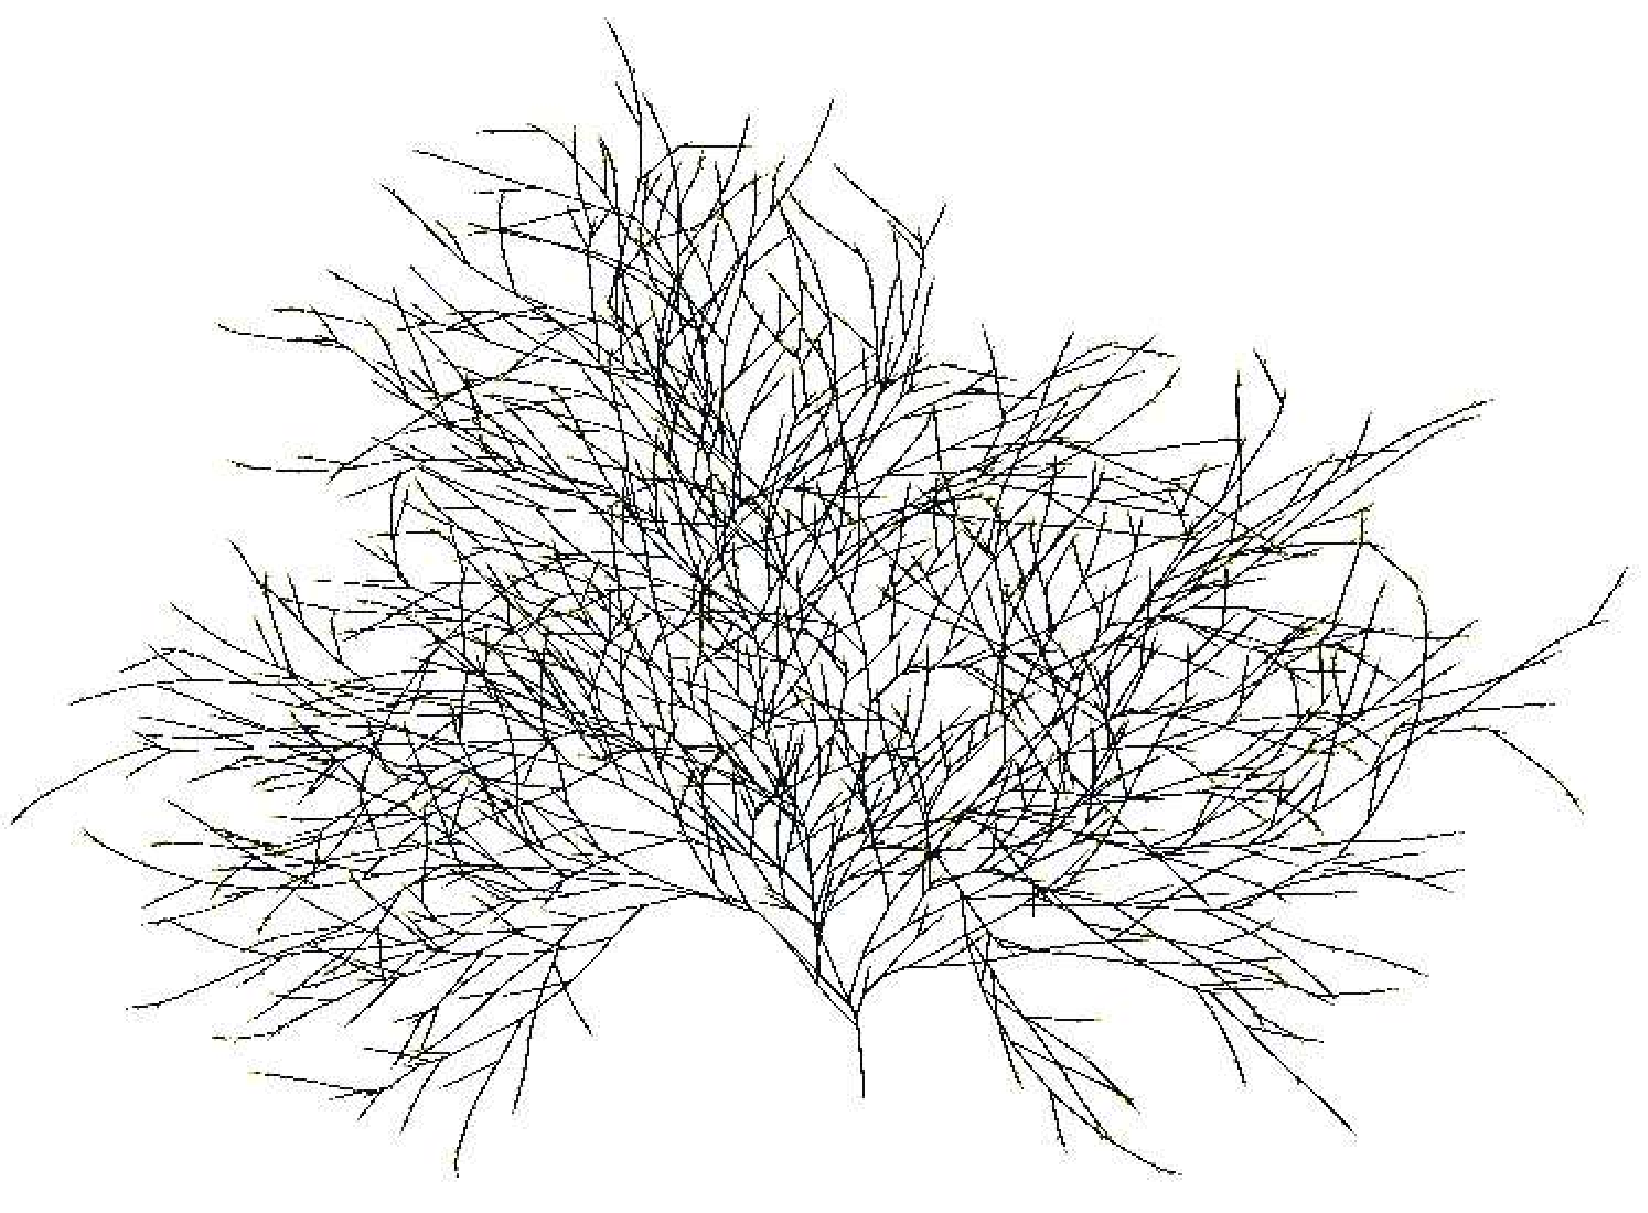
\includegraphics[scale=0.15]{auvaursi-sandpit-15-35d-30cm}
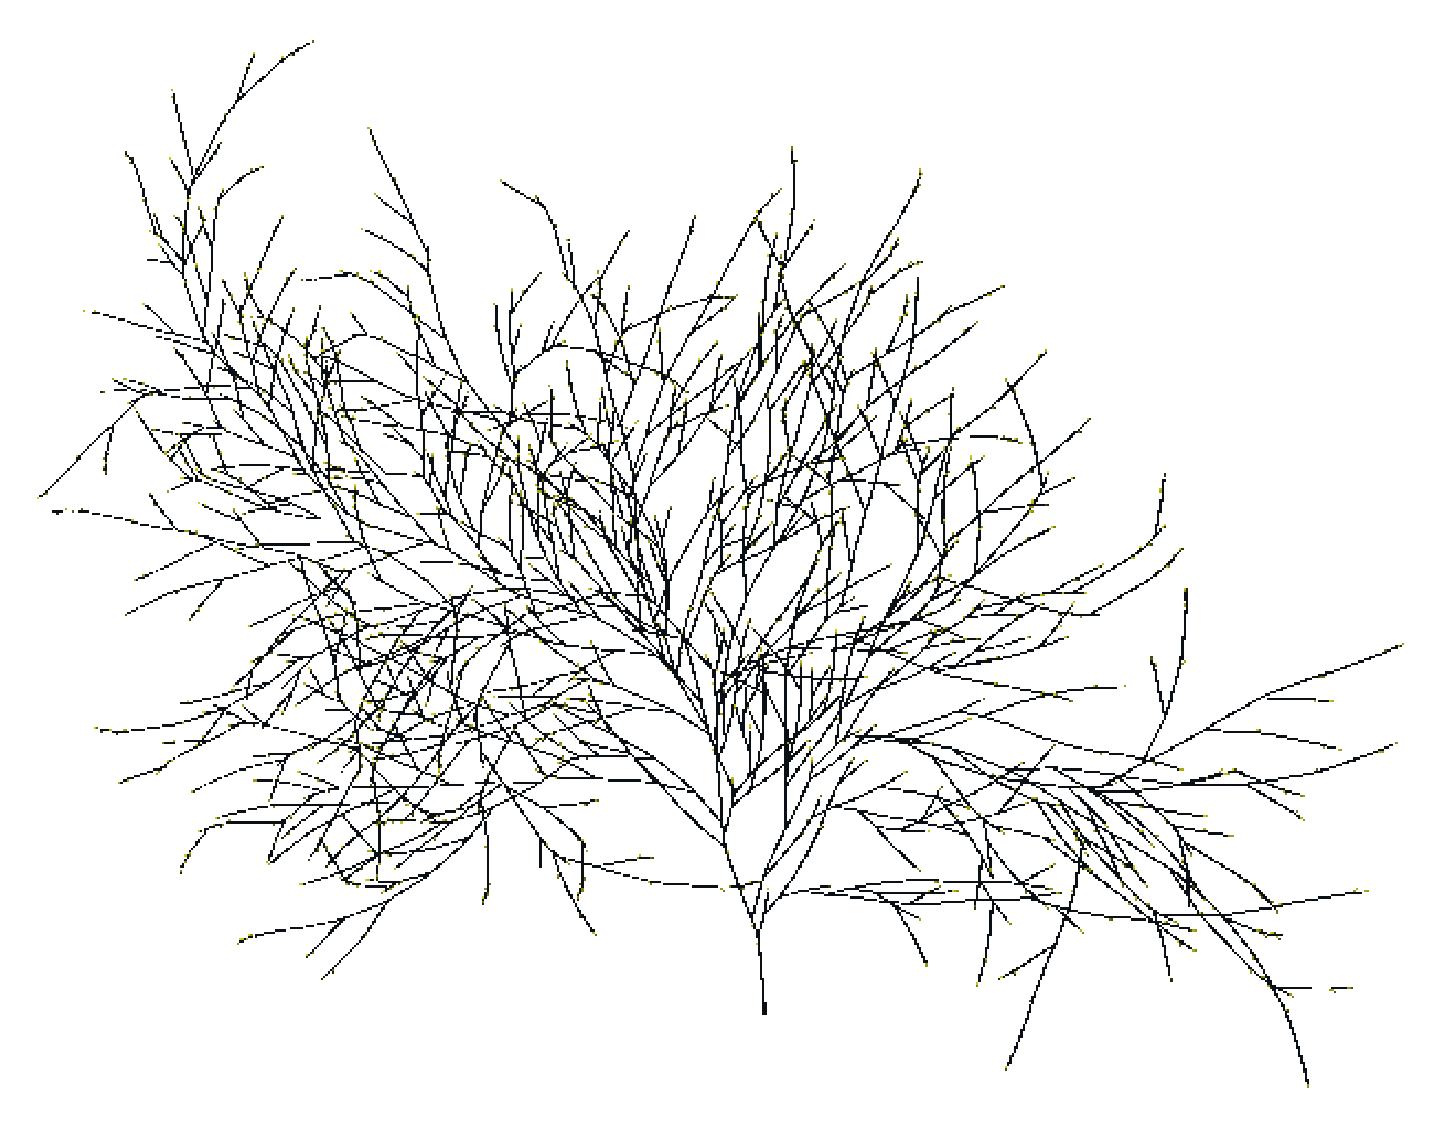
\includegraphics[scale=0.15]{auvaursi-sandpit-15-45d-30cm}
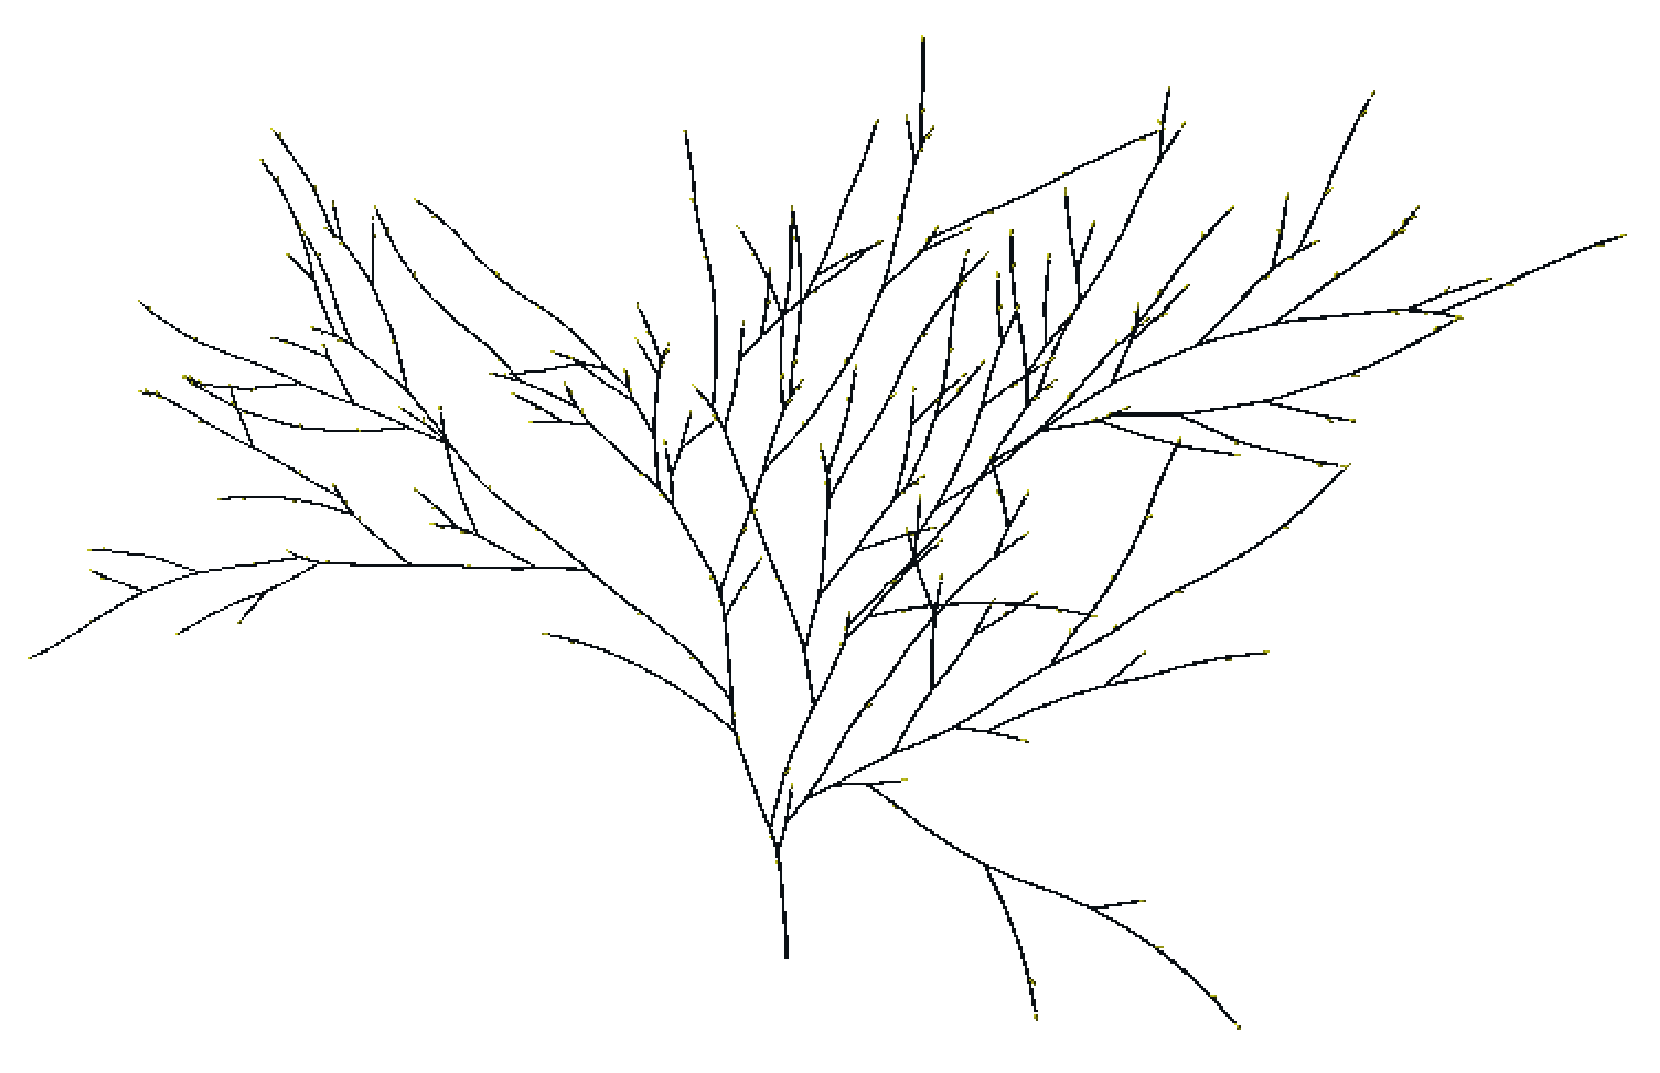
\includegraphics[scale=0.15]{auvaursi-sandpit-15-65d-30cm}    
\caption{The realization of the bearberry model by \citet{salemaa:02}
with the connection of L language program of Appendix \ref{sec:L2} and
LIGNUM.   The collision  detection is  accomplished by  LIGNUM.  Three
simulations  with 15  iterations using  different  collision detection
parameters for active buds. From  left to right: the opening angle and
the  distance  to  obstructing branch  are  $35^{\circ}/30\mathrm{cm},
45^{\circ}/30\mathrm{cm}$        and        $65^{\circ}/30\mathrm{cm}$
respectively.}\label{fig:a-uva-ursi}
\end{figure}
